%%%%%%%%%%%%%%%%%%%%%%%%%%%%%%%%%%%%%%%%%%%%%%%%%%%%%%%%%%%%%%%%%%%%%%%%%%%%
\begin{figure}[t]
\begin{center}
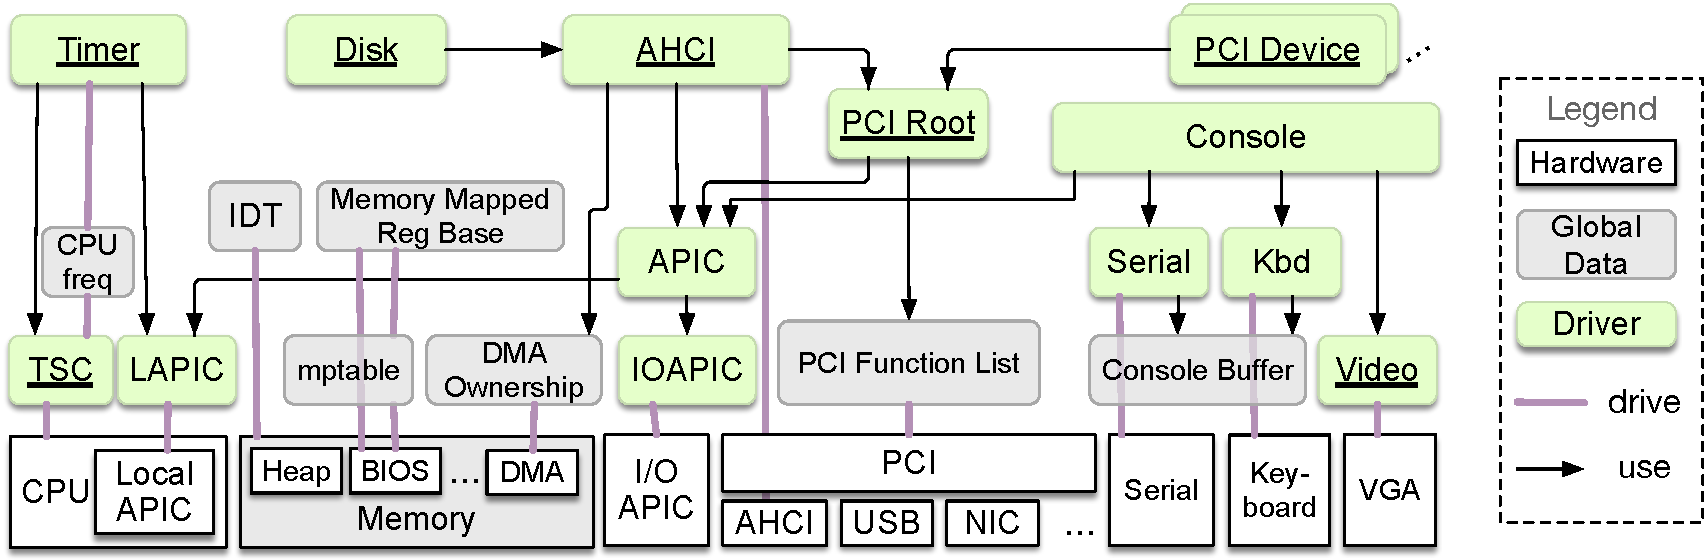
\includegraphics[width=0.95\textwidth]{figs/devices}
\end{center}
\caption{The device driver hierarchy of mCertiKOS}
\label{fig:overview:device}
\end{figure}
%%%%%%%%%%%%%%%%%%%%%%%%%%%%%%%%%%%%%%%%%%%%%%%%%%%%%%%%%%%%%%%%%%%%%%%%%%%%

In this chapter, we present a novel technique on how we can extend
our layer-based technology presented in Chapter \ref{chapter:framework}
to support verification of device drivers and interrupts.
We start from the existing mCertiKOS verified kernel presented in
Chapter \ref{chapter:sequential}. 
The kernel currently runs on the 32 bit x86 architecture.
It provides a multi-processing environment for user-level applications
using separate virtual address spaces. It implements both message
passing and shared memory inter-process communication protocols. As a
hypervisor, it can also boot recent versions of unmodified Linux
operating systems inside a virtual machine.  Unlike large commercial
operating systems like Linux or Unix, the mCertiKOS kernel only implements
a small subset of the POSIX-like API, e.g., process creation and
control, physical and virtual memory management, and
inter-process communication. It does
not implement signals, pipes, {\it etc}. The current file system
implementation in mCertiKOS is not verified. 

Figure~\ref{fig:overview:device} shows the device hierarchy of mCertiKOS. Here
the white boxes represent raw hardware devices; the green boxes denote the
device drivers, and the gray boxes are the data structures used by the drivers.
The purple/black lines show how these device and driver components are related.
Note that the drivers in mCertiKOS are not verified; they are implemented in
about 1,600 lines of C and assembly code and would be considered as part of the
trusted computing base (if they are kept inside the kernel). 

We take mCertiKOS's lowest level machine model, {\it LAsm}, and extend it with
device models. We model devices as finite state transition systems interacting
with the processor and the external environments. Since devices run concurrently
with the processor, parts of the device state change without the processor
explicitly modifying them. Though these ``volatile'' device states can change
nondeterministically, the processor itself only ever observes a ``current''
state when it reads the device data via an explicit I/O operation. The processor
does not, and in fact, {\it cannot} care about any states that the device may
enter between these observed states. Therefore, instead of designing
fine-grained small-step transition systems that model all possible interleaved
executions amongst the processor and devices, our devices simply perform an
atomic big-step transition whenever they are observed, i.e., when there is a
device read/write operation from the CPU.

Next, the machine model needs to be extended with the hardware interrupt
model. The processor responds to an interrupt by temporarily
suspending the current execution and then jumping to another routine
(i.e., an interrupt handler).  Interrupts can be triggered by both
hardware and software. Software interrupts (e.g., exceptions, system
calls) are relatively easy to reason about, since their behaviors are
always deterministic. For example, a page fault exception occurs
whenever the accessed address belongs to an unmapped page or a page
with wrong permission, and a system call is triggered by an explicit
instruction. However, hardware interrupts (IRQs) are unpredictable;
when we execute some code with interrupts turned on, at every
fine-grained processor step, the machine state (e.g., registers and
memory) may undergo significant changes.  Recent work on verified
operating systems (including mCertiKOS) neglects this kind of
reasoning, ignoring one of the largest kernel threat-surfaces
\cite{dscal15,klein2009sel4,Alkassar:VSTTE2010-71}.  Finally, modeling
interrupts is important because it also opens the way toward enabling
interrupts within the kernel.

\ignore{Recent work on verified operating systems (including
  mCertiKOS) avoid this kind of reasoning by either disabling
  interrupts throughout the kernel, or by polling the interrupts at a
  small number of carefully-placed interrupt points
  \cite{dscal15,klein2009sel4,Alkassar:VSTTE2010-71}. Disabling
  interrupts like this leads to a larger interrupt processing
  latency. \josh{also avoiding exceptions in the kernel eliminates
    optimizations like copy-on-write}}

\ignore{ We have developed a framework that supports reasoning of the
  device drivers and the rest of the kernel with potential interrupts
  at arbitrary execution point except in the interrupt handlers. In
  this subsection, we first present our interrupt model at the
  hardware level. Then we show how we gradually refine this low level
  interrupt machine model into the desired higher level one with
  interrupt handlers, where the reasoning of interruptible code can be
  naturally achieved.  }

On top of this lowest-level machine model, each kernel module can be
related to either device drivers (denoted as {\it DD}) or the rest of
the kernel (denoted as {\it K}, representing non-device-related kernel
components).  To introduce, verify, and abstract each such kernel
module into an abstract object with atomic logical primitive
transitions, we need to prove the following isolation properties:
\begin{itemize}
\item For each function in {\it K} or user space, which has interrupts
  turned on, the interrupt must not affect the behavior of the
  function. Although the code can be interrupted at any moment, and
  the control flow transferred to a place outside the function, it
  will eventually return with states (which the function relies upon)
  unchanged.

\item Devices which directly change the memory through Direct Memory
  Access (DMA), do not change any memory that the execution of any
  function in {\it K} depends on.

\item For each interruptible device driver function in {\it DD}, any interrupt
not related to the current device must not change any state related to the
current device.

\item In case that all interrupts related to a device are masked out, no 
interrupts can affect 
the state of the interrupt handler for the device.
\end{itemize}

For a particular fixed set of functions, the proof of the above
properties may not seem hard. However, they have to be proven
repeatedly for all possible combinations of currently introduced sets
of functions and devices. This immediately makes the verification of
an interruptible operating system with device drivers
unscalable. 

\begin{figure}[t]
	\begin{center}
		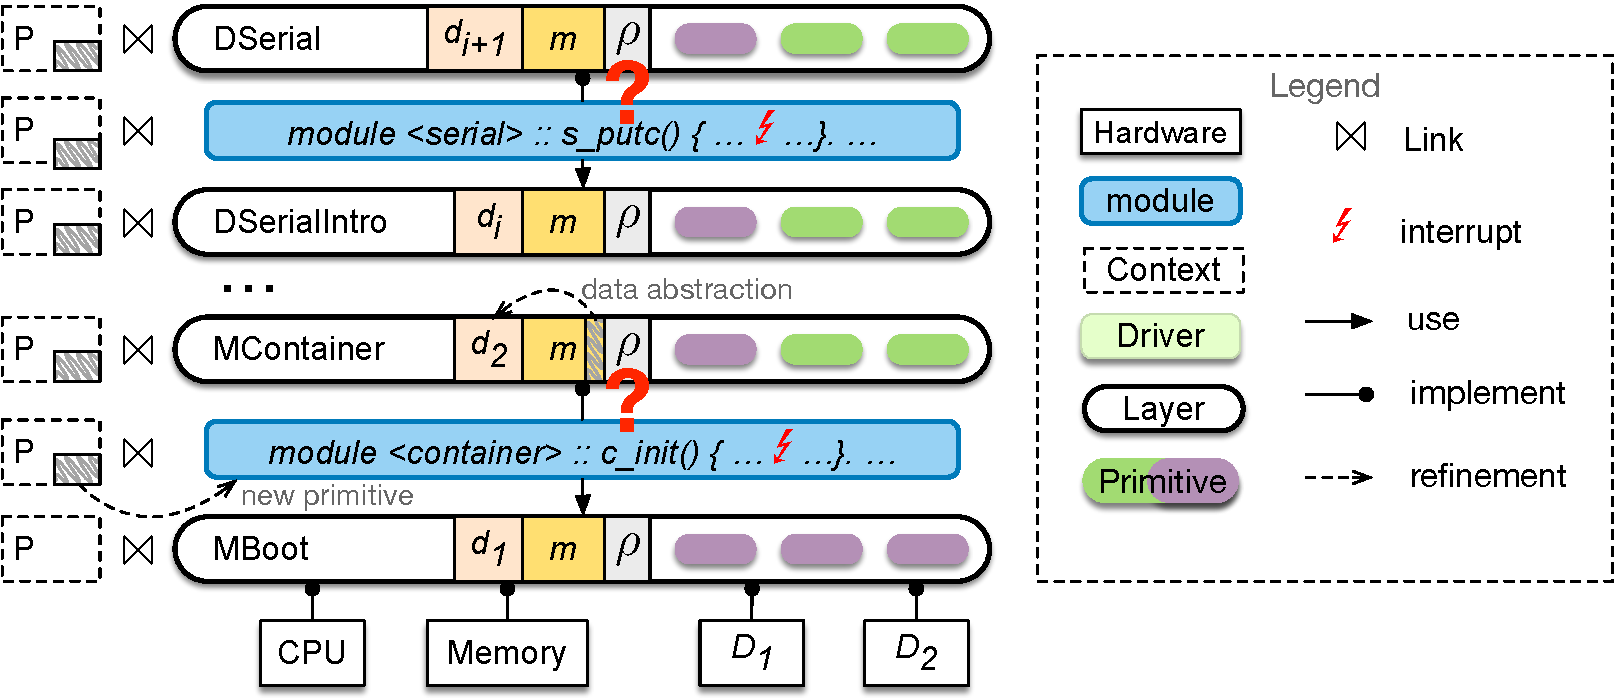
\includegraphics[width=0.95\textwidth]{figs/layer_pre}
	\end{center}
	\caption{Abstraction layers w. interrupts: a failed attempt}
	\label{fig:layer_pre}
\end{figure}

Furthermore, it is not obvious how to apply the techniques presented
in section \ref{chapter:framework}
to handle hardware interrupts. Figure~\ref{fig:layer_pre} shows one
such attempt.  Here, $\textsf{P}$ denotes the kernel/user-level
context code; $\textsf{MBoot}$, $\textsf{MContainer}$,
$\textsf{DSerialIntro}$, and $\textsf{DSerial}$ denote several kernel
and driver layers.  With interrupts turned on in the kernel, it is
immediately unclear how to show contextual refinement among different
layers. For a kernel function like $\textsf{c\_init}$, it cannot be
easily refined into an atomic specification as the code can be
interrupted at any point during the execution by a device interrupt
unless all possible interleavings of interrupts are encoded into the
specification itself. Similarly, for a device driver function like
$\textsf{puts}$, the code can be interrupted at any moment by
interrupts triggered by other devices or the device itself.

\ignore{In our hardware model, the states of CPU (registers and
  memory) and the states of v each device (device registers and
  internal hardware buffers) are strictly isolated. Thus, reasoning
  about their state transitions can be performed separately.}

\ignore{ Each device, together with associated device driver
  primitives and the interrupt handler, are connected with the
  processor in a certain way. The device has pieces of memory that it
  can access, while the device drivers normally have their own data
  stored in memory, e,g, buffers, FIFO queues, {\it etc}. Though they
  seem to be interconnected with the CPU through the memory, if you
  view the combined entity as a whole, it is strictly isolated from
  the entities of other devices, and the rest of the kernel.  The
  purpose of the above detailed properties are used to show that they
  are indeed isolated.  }

In this paper, we propose a systematic way that strictly
enforces isolation among different entities by construction.
Our approach consists of the following two key ideas. 

First, rather than viewing drivers as separate modules that interact
with the CPU via in-memory shared-state, we instead view each driver
as an extended device.  We utilize abstraction layers and contextual
refinement to gradually abstract the memory shared between a device
and its driver into the internal abstract states of a more general
device. Furthermore, we use the same technique to abstract those
driver functions that manipulate these data into the abstract
primitives of a higher level device. After this, our approach ensures
that those abstract states can no longer be accessed by the other
entities, through, e.g., memory reads and writes, but, rather, can
only be manipulated via explicit calls to the device interface. We
repeat these procedures so we can incrementally refine a raw device into
more and more abstract devices by wrapping them with the relevant
device drivers (see Fig.~\ref{fig:driver}). In the rest of the
paper, we call this extended abstract device a {\it device object}, to
distinguish it from the raw hardware device. Note that in our model,
device objects are indeed treated similarly to raw devices, and both
have quite similar interfaces.
% We introduce this name so we can
% refer to the underlying hardware devices unambiguously.

\begin{figure}[t]
	\begin{center}
		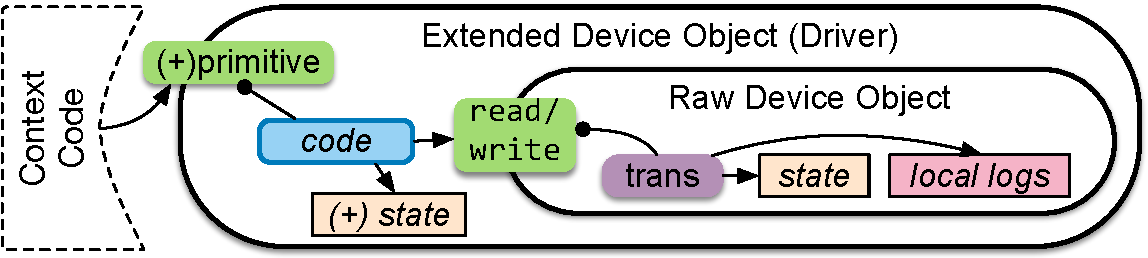
\includegraphics[width=0.75\textwidth]{figs/extends}
	\end{center}
	\caption{The driver as an extended device}
	\label{fig:driver}
\end{figure}

Second, we introduce and verify the interrupt handler for each device
at the lowest machine model, which is not yet suitable for reasoning
about interruptible code. This is possible because, for each device,
we require that either the interrupt be disabled or its corresponding
interrupt line be masked inside the
interrupt handler of the device. Next, we introduce a new abstract
machine with a more abstract interrupt model, that provides strong
isolation properties amongst different device objects and the kernel,
in which any future (context) code with interrupts turned on can be
reasoned about naturally. We prove a strong contextual refinement
property between these two abstract machines: any context code running
on the machine with the abstract interrupt model (overlay) retains an
equivalent behavior when it is running on top of the machine with the
concrete hardware interrupt model (underlay).

\begin{figure}
	\begin{center}
	  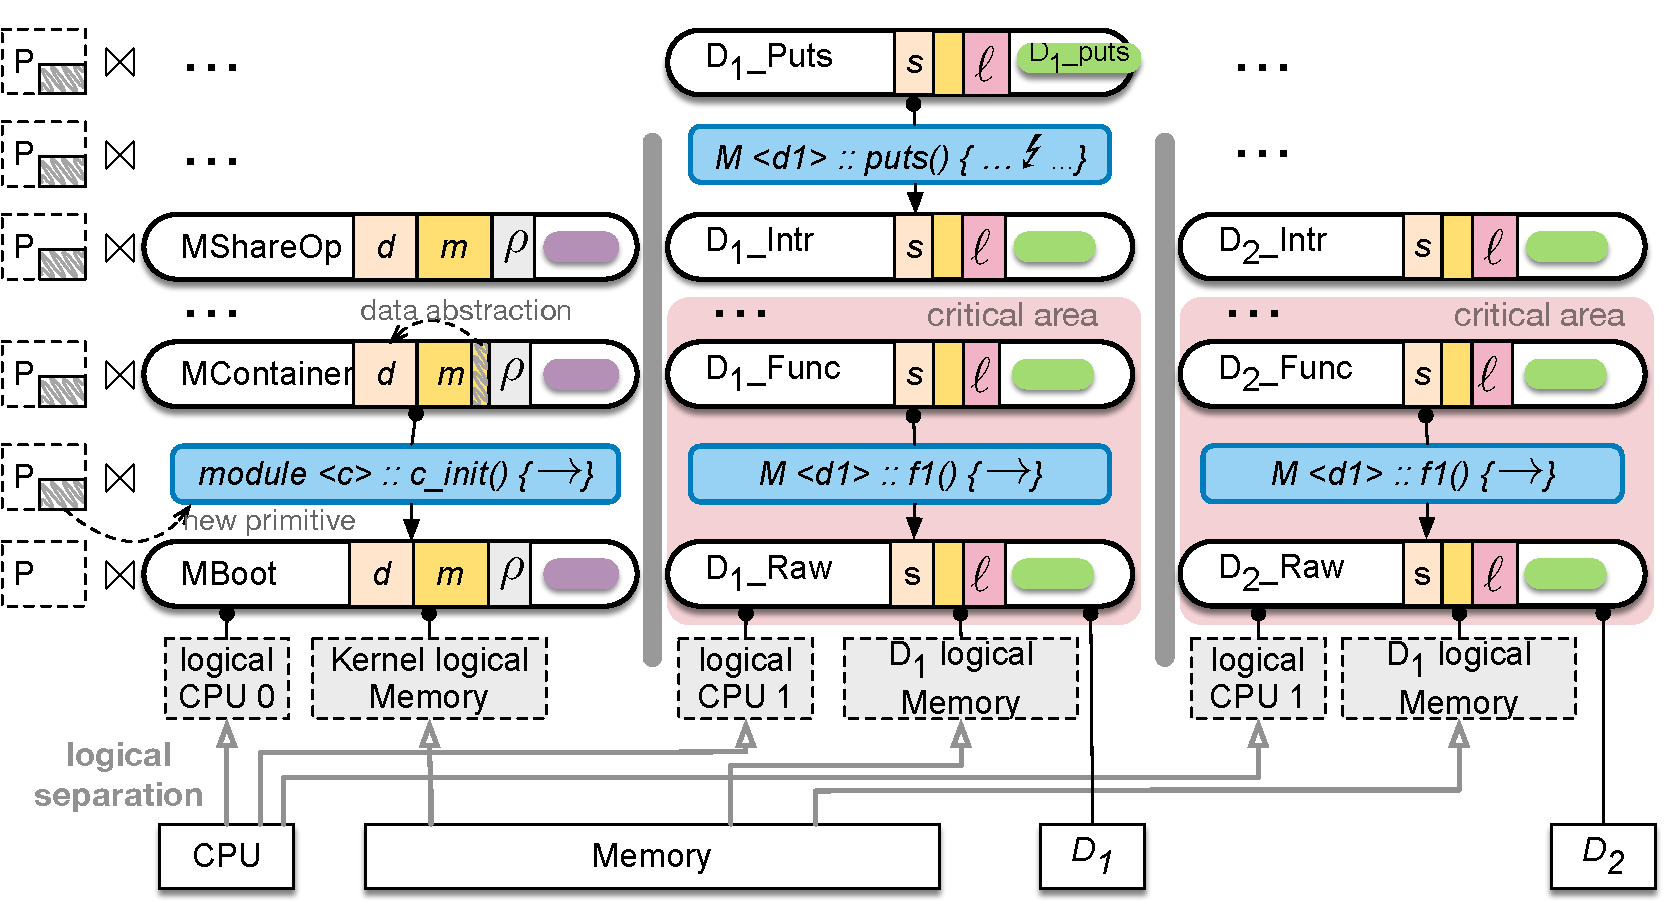
\includegraphics[width=0.90\textwidth]{figs/layer_new}
	\end{center}
	\caption{Building certified abstraction layers with hardware interrupts: our new approach}
	\label{fig:layer_new}
\end{figure}


Figure~\ref{fig:layer_new} shows the layer hierarchy of our
interruptible kernel with device drivers.  We treat the driver code as
if it runs on its own device's ``logical CPU,'' and each logical CPU
operates on its own separate internal states. Thus, the approach
provides a systematic way of assuring isolation among different device
objects (running on its own local logical CPUs) and the rest of the kernel.

On the kernel side (the layer hierarchy on the left hand side of
Fig.~\ref{fig:layer_new}), the contextual refinement is achieved in
the same way as shown in section \ref{chapter:framework} since the hardware interrupts (from
the other logical CPUs with separate states) no longer affect the
execution of any kernel primitive (like $\textsf{c\_init}$), i.e., the
kernel is completely interrupt-unaware.

Similarly, the device driver functions are no longer affected by the
hardware interrupts triggered from other devices.  For each device $D$
running on top of its own logical CPU, we first introduce and verify
part of the driver in the {\em critical area}, i.e., the low-level
device functions that should not be interrupted by the same device,
and the interrupt handler of the device.  Next, we use contextual
refinement to introduce a new layer that has a more abstract interrupt
model. On this layer, we can introduce and verify even interruptible
driver code (e.g., $\textsf{puts}$) while still enforcing strong
isolation and providing a clean interface to the kernel.

The rest of this chapter is organized as follows.
Sec.~\ref{sec:model} defines a formal machine model
extended with raw hardware devices. Sec.~\ref{sec:driver} presents
the device objects, hardware interrupt model, and abstract
interrupt model, and shows how we prove contextual refinement between
the two interrupt models. Sec.~\ref{sec:case_study} shows the Case study
of our verified drivers using the techniques developed in this
chapter, while Sec.~\ref{sec:layers} presents concrete
Coq implementations of certified abstraction layers.
Sections~\ref{sec:lessons} gives an evaluation of our new techniques
and describe the lessons we learned.

\ignore{ At the machine level, the interface between the CPU execution
  and the device state transition is fairly clear. The CPU
  communicates with devices through e.g., I/O instructions, memory
  mapped I/O, while the device interacts with CPU with interrupts,
  Direct Memory Access (DMA), {\it etc}. The executions of the
  programs that do not communicate with devices are isolated to those
  of devices', thus can be reasoned separately.

The very purpose of an operating system is to provide an
abstract device interface to its users. 
Unfortunately, as soon as some device driver code are introduced
in the kernel, it immediately blurs the clean interface between the
operating system and devices. This is because the execution of the
kernel code and transitions of devices are interrelated, i.e., each
side may affect the other one's behaviors, thus making the modular
reasoning extremely complicated. Consider a very simple kernel
function $f$ that copies a small fragments of some device data into some
memory through the device interface, e.g., I/O instructions, memory mapped
I/O, {\it etc}. This preliminary function can
be used in another kernel function to implement a more complex
operation. However, invocation of $f$ affects
both the kernel execution (it modifies memory, thus changes the behavior
of other kernel code depends on this part of memory) and the device
transition (it interacts with devices).  Even worse, some functions may
manipulate several devices simultaneously, e.g., a debug function in a
console driver may write to both the serial port and the display.
This means the kernel execution may affect the transitions of multiple
devices in a rather complex manner. On the other hand, the devices can
also change the behaviors of kernel executions. For the parts of the
kernel with interrupts turned on, devices can interrupt the kernel execution
by an interrupt, force moving the kernel's execution to somewhere else.
When it returns, there is no formal guarantee that the states that the current
execution relies on are not changed by someone else. Furthermore, devices
can also directory change some designated parts of memory through DMA.
The reasoning in this model is complicated as, in theory, any kernel execution
may affect device transitions and any devices may change the behaviors of the
kernel execution. It would be ideal if the two entities are completely isolated
even at very high level of abstractions in the kernel, and the communication
is only done through some clearly specified interfaces that only affects
behaviors of single responsible entity.

In \cite{dscal15}, the authors present a compositional framework to
incrementally build the layers of abstractions
through the notion of contextual refinement, which they apply to
the verification of a practical operating system called mCertiKOS
as a case study.
We extend this framework to build a more powerful framework which
supports a general notion of devices, and compositional verification
of device drivers. One key idea is to broaden the notion of a device.
In our machine model, a ``device'' is no longer limited to a
physical device, but is an abstract representation of one or more
devices together with the functions manipulating those devices.
One observation is that the device drivers,
although could be interconnected in complex ways, are rather isolated from
the rest of operating system (This is not true if the device drivers call sleep or
yield. What should we say about this???). For example, when a serial driver copies
the received serial characters from the serial device into a serial buffer, this
serial buffer stored in memory should be private to the serial driver.
Any good implementation practice of other kernel modules should not directly
access this serial buffer, but through the clean interfaces
provided by the serial driver. In our approach, we view the transitions performed
by the device driver code part of the device transitions. This novel view allows
us to incrementally wrap a physical device with driver code
to build more and more abstract notion of devices, utilizing the idea of
abstraction layers and contextual refinement, while strictly enforcing
isolation between the kernel and ``devices''.

In the case of example above, we utilize the technology presented in \cite{dscal15}, 
to introduce a new abstraction layer on top of the current layer that abstracts
the memory that $f$ manipulates at underlay into an abstract representation
of the same data at overlay. In this framework, abstract states are opaque
to the kernel, and cannot be accessed through regular CPU instructions like
memory operations. The contextual refinement proof between these two abstraction
layers guarantees that the actual information saved in the memory at underlay
and the corresponding abstract representation in the abstract states of overlay
are always related for all possible context code running on the machines,
e.g., more device drivers, any kernel extensions, user programs, {\it etc}.
Then at overlay, we combine this new abstract state with the original device state
to form the state of the new abstract device at overlay, and add $f$ as the
new interface of the new device. Any existing interfaces of original device
at the underlay can be
passed through to the overlay or can be hidden. This can be done for each
device if they do not interfere with each other.
In the case where the newly introduced function interacts with multiple devices,
or multiple devices interfere among each other at the current layer, we merge
these interacting components into a single abstract heterogeneous device.

On the other hand, devices may still affect kernel behaviors, e.g., through
DMA or interrupts. In the case of DMA, we can take similar approach to
abstract the corresponding memory into device abstract states, and incrementally
build more abstract devices through abstraction layers by embarrassing
more and more code that manipulates corresponding devices and memory.
On the other hand,
addressing the issues caused by device interrupts is more complex because,
even in our model above, it is not clear why the device interrupts would
not cause any kernel's states to change. This becomes clear only when 
the interrupt handlers for the devices of interests are fully specified
and verified. At that moment, we have full formal specifications of
behaviors of the device interrupts which can be used to prove the isolation
of kernel execution from device interrupts. In our approach, we perform the
verification of device interrupt handlers as early as possible, and
requires that for these code that run in the very low level of abstraction,
the interrupts are always turned off, e.g., during the execution of device drivers.

Our approach guarantees that any kernel execution would not affect device
transitions except through the well specified interfaces, any device transitions
cannot change the behaviors of kernel execution even in the presence of device
interrupts. Majority of the device driver code in our system are written in C
and verified at the C level, and both the code and the proof are compiled down
to the assembly level through a modified version of the CompCert verified
compiler \cite{dscal15}. With this clean interface enforced by our compositional
framework, reasoning even at a higher level language like C is no longer scary.
During the building of the device hierarchy, the reasoning can be done locally
without worrying about any nondeterministic interference from the original
kernel. We also do not have to change any existing C level proof related to the
kernel in the mCertiKOS, which is completely interrupt-unaware, thanks to this
nice isolation between two entities. (We are gonna insert a figure here to
further illustrate the idea.)

There is still one remaining issue. Majority of our device drivers
are verified at C level. On the other hand, hardware devices run
inherently concurrent to CPU, thus so does our general notion of devices to
the kernel. \newman{Here I am gonna explain our idea of lazily performing
the transitions of each device, logs, and so on. Basically the stuff we do
to determinize the semantics at the C level. I will also talk about
the relation between this deterministic machine to the realistic
non-deterministic machine, and how we can? formally link those together
to illustrate our deterministic machine model is not unrealistic.}

}
